\documentclass[10pt,a4j,twocolumn]{jsarticle}

\usepackage[dvipdfmx]{graphicx}
\usepackage{url}
\setlength{\textheight}{275mm}
\headheight 5mm
\topmargin -30mm
\textwidth 185mm
\oddsidemargin -15mm
\evensidemargin -15mm
\pagestyle{empty}
\begin{document}
\title{RubyでMapleを動かすためのインターフェースの開発}
\author{情報科学科 西谷研究室 3528 村瀬愛理}
\date{}
\maketitle
\section{研究目的}
\vspace{-0.5em}
Rubyでは数値計算のライブラリ開発が遅れており,Ruby上では高等な関数(素数を求めたり,最小公倍数を求めるなど)を使った数式処理を行うのが難しい.また,Ruby以外の数式処理ソフトウェアを別に立ち上げて別々で作業したり,慣れない別の言語を勉強し直したりするよりも,Rubyのみでプログラミングする方が開発速度の格段の向上が期待できる.そこで本研究では,MapleをRuby上で呼び出し,Mapleに高等な関数や桁数の大きな数値を用いた計算をさせて,その結果をRubyが取得するインターフェースライブラリの開発を目的とする.

\section{手法}
\vspace{-0.5em}
\paragraph{Mapleとの連携}
Mapleは一般的に,グラフや数式の綺麗な出力や,数式の入力を初心者が直感的におこなえるようにJavaで作られたGUIを使って実行する.それとは別にcommand lineで実行される計算エンジン部が用意されている.ここで開発するRubyライブラリでは,このエンジンに直接働きかけて操作する.Rubyで外部コマンドを実行するgem libraryのsystemuを使って,出力を得るようにしている.Ruby codeで要求コードを受け取った場合,そのコードをtmpファイルに書き込む.それをMapleで実行し,結果をテキストファイルで受けとり出力を得る.

\paragraph{Maple関数の類型化}
今回,数多く存在するMapleの数学関数の中から整数論と行列に関するものを選抜し実装した後,入出力に関して類型化し,それぞれの出力に応じてwrapperを作った.表1は類型化の一部である.
\begin{table}[htbp]\begin{center}
\caption{実装した整数論に関する関数と入出力.}
\label{table:one}
\begin{tabular}{lllll}
\hline
関数名  &振る舞い  &入力型  &出力型  \\ \hline
nextprime  &次の素数を求める  &int  &int  \\
lcm  &最小公倍数  &int, int  &int  \\
gcd  &最大公約数  &int, int  &int  \\
isprime  &素数判定  &int  &boolean  \\
\hline
\end{tabular}
\label{default}
\end{center}
\vspace{-2em}
\end{table}
%for inserting separate lines, use \hline, \cline{2-3} etc.

\section{基本動作}
\vspace{-0.5em}
入力された値の次の素数を出力するnextprimeを例に説明する.
\begin{figure}[htbp]\begin{center}
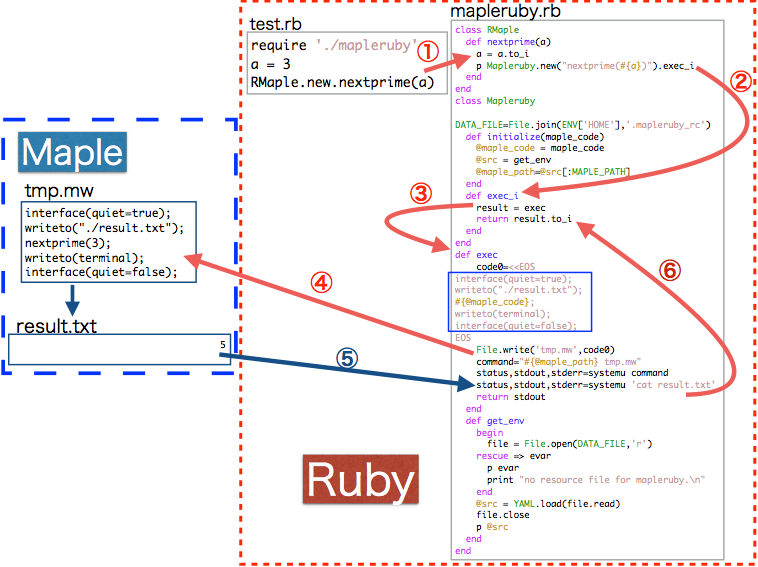
\includegraphics[width=7.7cm, bb=0 0 546 408]{./mapleruby_003.png}
\caption{maplerubyの基本動作.}
\label{default}\end{center}
\vspace{-2em}
\end{figure}
\begin{enumerate}
\item maplerubyをrequireした上で使いたい関数を呼び出す.RMaple.new.hogehogeのhogehogeに使いたい関数名(ここではnextprime)を入れる.
\item RMapleクラス内のnextprime関数が呼び出される.その後,Maplerubyクラスのexec\_i関数へ"nextprime(3)"が出力される.この出力された文字列がそのままMapleでの計算に使われる.
\item 出力された文字列をさらにexec関数へ出力する.
\item 青四角内の内容をMapleへと出力する.この時\verb|#{@maple_code};|に先ほどの"nextprime(3)"が入る.青四角の内容がMapleに出力・実行されることで得られた答えがresult.txtに出力される.
\item result.txtに出力された内容をRuby側で受け取り,exec\_iに再び返す.
\item 返された値をto\_iすることでint型に直して解を出力する.
\end{enumerate}


\section{本研究による成果}
\vspace{-0.5em}
本研究で得られた成果をまとめると以下の通りである.
\begin{itemize}
\item RSA暗号化における計算が,Ruby単体で行うよりも約100倍の数まで扱えるようになった.
\item 3行3列の行列について逆行列や固有値,固有ベクトルを求めることができた.
\end{itemize}
従来では,MapleとRubyを行き来しなければならなかったような計算でも,maplerubyを用いることでRuby上のみで完結させられるようになった.

\section{総括}
\vspace{-0.5em}
Rubyだけで桁数の大きい計算や複雑な数学関数を必要とする計算が完結させられることが可能になった.今後は新たな関数の追加や,Mapleの特徴である綺麗なグラフ描画ができることを生かしたグラフの出力を可能にするなどが課題として挙げられる.

\end{document}
